\chapter{Finden eines Projektes}
Es existieren viele verschiedene Quellen, welche Anregungen zu 3D-Druck oder \ac{DIY} Projekten geben können oder bereits komplette Anleitungen zu Projekten beinhalten. Im Folgenden wird ein kurzer Überblick zu den bekanntesten Quellen gegeben.

\section{DIY-Webseiten}
Einen ausgezeichneten ersten Anlaufpunkt bieten \ac{DIY}-Seiten wie \textit{Instructables}\footnote{\url{https://www.instructables.com}}. Dort sind Projekte zu den verschiedensten Themen zu finden, es existiert aber auch ein eigener Bereich für 3D-Druck Projekte.

\section{Seiten für 3D-Objekt Austausch}
Eine weitere Möglichkeit bieten Webseiten für den Austausch von 3D-Objekten. Dort können von jedem die Dateien, welche zum Druck von 3D-Objekten benötigt werden, hochgeladen und von Anderen gefunden werden. Eine der bekanntesten freien Seiten ist \textit{Thingiverse}\footnote{\url{https://www.thingiverse.com}}. Es existieren allerdings auch Seiten auf welchen die entsprechenden Dateien zum Verkauf angeboten oder auch fertig gedruckt bestellt werden können, beispielsweise \textit{CGTrader}\footnote{\url{https://www.cgtrader.com}} oder \textit{Shapeways}\footnote{\url{https://www.shapeways.com}}.

\section{Herstellerseiten}
Auch einige Hersteller bieten auf ihren Seiten eigens auf ihre Produkte zugeschnittene Projekte an. Der Vorteil hier ist, dass im Normalfall keine Anpassungen an den Modellen vorgenommen werden müssen oder sogar direkt der entsprechende G-Code (Steuerbefehle für den 3D-Drucker) zur Verfügung steht. Ein Beispiel hierfür ist die \textit{Zortrax Library}\footnote{\url{http://library.zortrax.com}} des Herstellers \textit{Zortrax}, aus welcher auch das in dieser Arbeit behandelte Projekt stammt.

\begin{figure}[h]
  \centering
  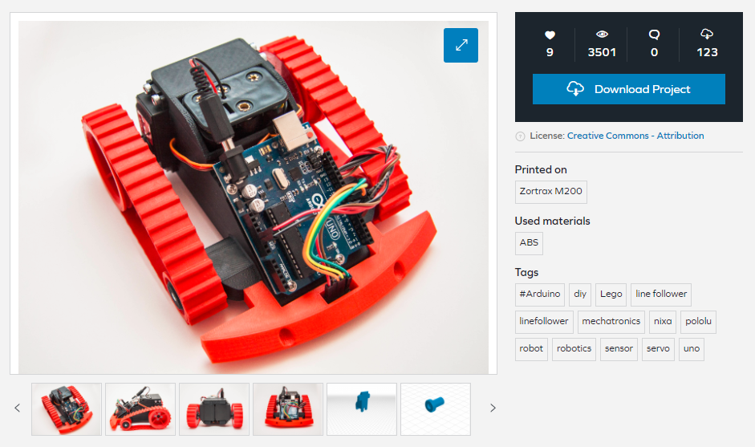
\includegraphics[width=10cm]{kapitel1/projekt}
  \caption{LineFollower Projekt aus der Zortrax Library}
  \label{Kap1:Projekt}
\end{figure}

\section{Printmedien}
Die letzte Mögliche Quelle für Projekte sind 3D-Druck oder \ac{DIY}-Printmedien. Im deutschen Raum gibt es hier bisher nur wenige Vertreter, der bekannteste davon die Zeitschrift \textit{Make:}\footnote{\url{https://www.heise.de/make/}}. Gelegentlich werden auch 3D-Druck Projekte in anderen Fachzeitschriften wie der \textit{c't}\footnote{\url{https://www.heise.de/ct/}} veröffentlicht.